% Permission is granted to copy, distribute and/or modify this document
% under the terms of the GNU Free Documentation License, Version 1.2
% or any later version published by the Free Software Foundation;
% with no Invariant Sections, no Front-Cover Texts, and no Back-Cover
% Texts.  A copy of the license is included in the section entitled "GNU
% Free Documentation License".
% Copyright 2015 EDF
%

%%%%%%%%%%%%%%%%%%%%%%%%%%%%%%%%%%%%%%%%%%%%%%%%%%%%%%%%%%%%%%%%%%%%%%%%%%%%%%%%%%%%%%%%%%
\section{Architecture guide}

This document makes up the general specification design for the general linear model stepwise regression analysis
in OpenTURNS.

\subsection{Linear regression models}

The \texttt{LinearModel} class is outdated and does not follow current best practices about metamodel classes.
We will introduce \texttt{LinearModelAlgorithm} and \texttt{LinearModelResult} classes.
All current uses of \texttt{LinearModel} have to be modified; it is used in classes \texttt{VisualTest},
\texttt{CorrelationAnalysis} and \texttt{LinearModelTest}. Class \texttt{LinearModelFactory} will be deprecated.

\begin{figure}[htb]
  \begin{center}
    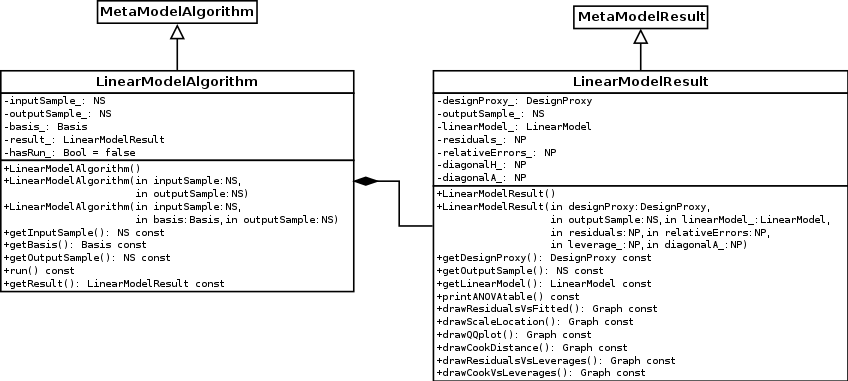
\includegraphics[scale=0.5]{LinearModelAlgorithm.png}
    \caption{LinearModelAlgorithm and LinearModelResult classes}\label{fig:archi:LinearModelAlgorithm}
  \end{center}
\end{figure}

\subsection{ANOVA table}

It is requested to give access to the following data:
\begin{itemize}
\item Linear model formula, in a textual form
\item Informations about residuals (minimum, maximum, median, mean, quantiles, standard deviation)
\item For each factor,
\begin{itemize}
\item its coefficient
\item its standard error
\item p-value for Student test
\item A visual symbol for significance test
\end{itemize}
\item Number of degrees of freedom
\item Coefficients $R^2$ and adjusted $R^2$
\item p-value of the Fisher test
\item normality tests on residuals (Kolmogorov-Smirnov, Anderson-Darling and $\chi^2$)
\end{itemize}

Note: Student test uses
\[
\frac{\hat{\beta}_i}{\sqrt{\frac{n}{n-p-1}\left[(X^T X)^{-1}\right]_{i,i}}}
\]

\subsection{Graphical diagnostics}

Several plots are provided by \texttt{LinearModelResult} class, see diagram class.
\begin{itemize}
\item \texttt{drawResidualsVsFitted} plots standardized residuals $\tilde{\epsilon}$ vs. fitted values, with
\[
\tilde{\epsilon}_i = \frac{\hat{\epsilon}_i}{\sqrt{\frac{n}{n-p-1}\hat{\sigma}^2 (1-H_{i,i})}}
\]
\item \texttt{drawQQPlot} plots $\sqrt{|\tilde{\epsilon}_i|}$ vs. theoretical quantiles.
\item \texttt{drawScaleLocation} plots $\sqrt{\tilde{\epsilon}_i}$ vs. fitted values.
\item \texttt{drawCookDistance} plots an histogram of Cook's distance
\[
D_i = \frac{\tilde{\epsilon}_i^2}{p} \left(\frac{H_{i,i}}{1-H_{i,i}}\right)
\]
\item \texttt{drawResidualsVsLeverages} plots standardized residuals $\tilde{\epsilon}$ vs leverages
\[
h_i = H_{i,i}
\]
Moreover, this plot also contains contour plot of function
\[
D(x,y) = \frac{y^2}{p}\left(\frac{x}{1-x}\right)
\]
for levels $0.5$ and $1$.
\item \texttt{drawCookVsLeverages} plots Cook's distance $\tilde{\epsilon}$ vs $\frac{h_i}{1-h_i}$.
\[
h_i = H_{i,i}
\]
Moreover, this plot also contains isolines of function
\[
\frac{py}{x}
\]
\end{itemize}

All these plots must display labels of some extremal points.  To this end, the following attributes
and methods will be added to \texttt{Cloud} and \texttt{BarPlot}:
to allow
\begin{verbatim}
   /** Setter for labels */
   Description getLabels() const;
   void setLabels(const Description & labels);
   /** Labels */
   Description labels_;
\end{verbatim}
The \texttt{labels} argument must have the same size as graph data, and only non-empty labels are
printed.

\texttt{LinearModelAlgorithm} derive from \texttt{MetaModelAlgorithm}, with standard pimpl idiom
as prescribed by OpenTURNS coding rules.

\begin{figure}[htb]
  \begin{center}
    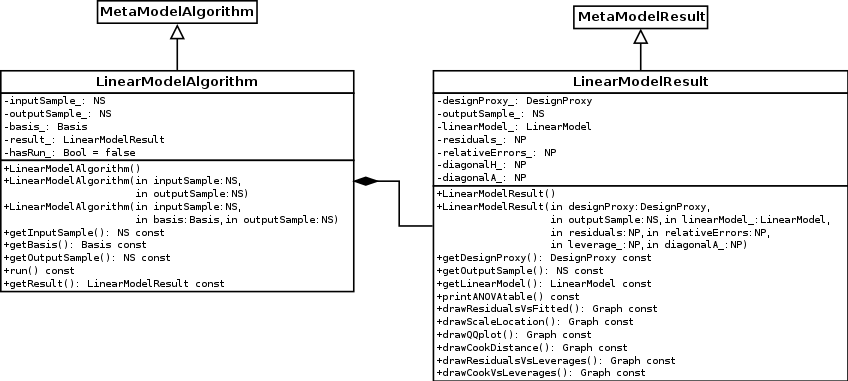
\includegraphics[scale=0.5]{LinearModelAlgorithm.png}
    \caption{LinearModelAlgorithm class}\label{fig:archi:LinearModelAlgorithm}
  \end{center}
\end{figure}

\subsection{Step method}

\texttt{LinearModelStepwiseAlgorithm} derive from \texttt{PersistentObject}
\begin{figure}[htb]
  \begin{center}
    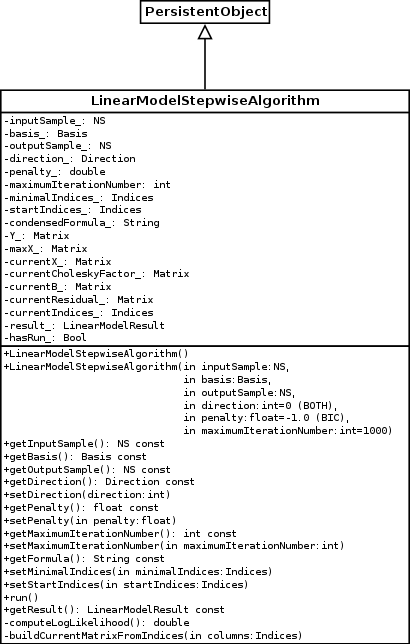
\includegraphics[scale=0.5]{LinearModelStepwiseAlgorithm.png}
    \caption{LinearModelStepwiseAlgorithm class}\label{fig:archi:LinearModelStepwiseAlgorithm}
  \end{center}
\end{figure}
